\RequirePackage[ngerman=ngerman-x-latest]{hyphsubst}
\documentclass[
        ngerman,
        paper=a4,
        numbers=noendperiod,
]{scrreprt}
\setcounter{secnumdepth}{3}
\setcounter{tocdepth}{3}
% Encoding
\usepackage[utf8]{inputenc}
\usepackage[T1]{fontenc}
% Sprachsupport
\usepackage[ngerman]{babel}
\usepackage{translator}
% Tabellen
\usepackage{booktabs}
\usepackage{tabularx}
\usepackage{pdflscape}
\usepackage{multirow}
% Symbole
\usepackage{eurosym}
% Formeln
\usepackage{amsmath, amsthm, amssymb}
% Formelregeln
\DeclareNewTOC[% 
  counterwithin=chapter, 
  indent=0pt,% kein Einzug im Verzeichnis 
  hang=2em,% Einzug für den Text im Verzeichnis 
  name=equation, 
  type=xequation, 
  nonfloat, 
]{loe} 

\AtBeginDocument{% 
  \newcaptionname{ngerman}\xequationname{Formel}% 
  \newcaptionname{ngerman}\listxequationname{Formelverzeichnis}% 
} 
% Pakete
\usepackage{amsthm}
\usepackage{float}
\usepackage{wrapfig}
\usepackage[babel,german=quotes]{csquotes}
\usepackage[square,sort]{natbib}
\usepackage[hyphens]{url}
\usepackage{setspace}
\onehalfspacing
\usepackage[
        pdftex,
        hyperfigures,
        hyperindex,
        bookmarksnumbered,
        linktoc=all,
        pdfborder={0.25 0.25 0.25},
        %pdfborder={0 0 0},
        pdfpagelayout=TwoColumnRight,
]{hyperref}
\usepackage[all]{hypcap}
\usepackage{lmodern}
\usepackage[final,babel]{microtype}
\usepackage{graphicx}
\usepackage{fancyhdr}
\usepackage[printonlyused]{acronym}
\usepackage{subfiles} 

\pagestyle{fancy}
\renewcommand{\chaptermark}[1]{\markboth{#1}{}}
\fancyhf{}
\fancyhead[RE]{\chaptername~\thechapter}
\fancyhead[LO]{\leftmark}
\fancyhead[LE,RO]{\thepage}

%Quellcodes
%Farben
\usepackage{color}
\definecolor{dkgreen}{rgb}{0,0.6,0}
\definecolor{gray}{rgb}{0.5,0.5,0.5}
\definecolor{mauve}{rgb}{0.58,0,0.82}
%Listing einfaerben
\usepackage{listings}
\lstset{numbers=left,
	numberstyle=\tiny,
	numbersep=5pt,
	breaklines=true,
	showstringspaces=false,
	frame=l ,
	xleftmargin=15pt,
	xrightmargin=15pt,
	basicstyle=\ttfamily\scriptsize,
	stepnumber=1,
	keywordstyle=\color{blue},          % keyword style
  	commentstyle=\color{dkgreen},       % comment style
  	stringstyle=\color{mauve}         % string literal style
}
%Sprache Festelegen
\lstset{language=R}

\begin{document}
\begin{titlepage}
    \begin{center}
    \huge \textbf{\textsf{Implementierung eines QA-Bot-Prototypen aus Wikipedia Zusammenfassungen}} \\
    \vspace{1cm}
    \LARGE\textbf{\textsc{Projektarbeit }}\\
    \vspace{1cm}
    \normalsize
    vorgelegt am: \today \\
    \vspace{2.5cm}
    \large \textbf{Fakultät IV - 
Institut für Wissensbasierte
Systeme und Wissensmanagement, Universität Siegen
}
\linebreak
\linebreak
\begin{figure}[H]
    \centering
\includegraphics[width=0.4\linewidth]{images/imageuni.pdf}
    \label{fig:Unilabel}
\end{figure}
    \end{center}
    \vspace{3cm}
    \begin{center}
 \normalsize{
    \begin{tabular}{ll}
    	Eingereicht von: & {Ugur Tigu} \\
    	Studiengang: & Wirtschaftsinformatik, Master of Science (M.Sc.)\\
	Erstprüfer: & Prof. Dr.-Ing. Madjid Fathi \\
	Betreuer: &   Johannes Zenkert\\
    \end{tabular}\\
    }
\end{center}
\end{titlepage}
\setcounter{page}{0}
\pagenumbering{Roman}
\tableofcontents
\clearpage 
\addcontentsline{toc}{chapter}{Abbildungsverzeichnis}
\listoffigures
\clearpage 
\addcontentsline{toc}{chapter}{Tabellenverzeichnis}
\listoftables
\clearpage 
% Kapiteldefinition ohne Nummerierung
\chapter*{Abkürzungsverzeichnis}
 % Abkürzungsverzeichnis soll im Inhaltsverzeichnis erscheinen
\addcontentsline{toc}{chapter}{Abkürzungsverzeichnis} 
\begin{acronym}
% Format der Abkürzungsdefinition: \acro{}[]{}
% {Verweis}[Abkürzung]{ausgeschriebene Abkürzung}

\acro{nlp}[NLP]{Natural Language Processing}
\acro{qa}[QA]{Question Answering}
\acro{ir}[IR]{Information Retrieval}
\acro{pos}[POS]{Part-of-speech}

\end{acronym}
\clearpage 
\addcontentsline{toc}{chapter}{Formelverzeichnis} 
\listofxequations
\clearpage
\addcontentsline{toc}{chapter}{Listings} 
\lstlistoflistings
\clearpage
\setcounter{page}{1}
\pagenumbering{arabic}


%%%%%%%%%%%%%%%%%%%%%%%%%%%%%%%%%%%%%%%%%%%%%%%%%%%%%%%%%%%%%%%%%%%%%%
%3 Seiten
\chapter{Einleitung}
\section{Motivation}
\section{Forschungsfragen}
\section{Struktur der Arbeit}
%%%%%%%%%%%%%%%%%%%%%%%%%%%%%%%%%%%%%%%%%%%%%%%%%%%%%%%%%%%%%%%%%%%%%%

%%%%%%%%%%%%%%%%%%%%%%%%%%%%%%%%%%%%%%%%%%%%%%%%%%%%%%%%%%%%%%%%%%%%%%
% 24 Seiten
\chapter{Theoretische Grundlagen}
%%%%%%%%%%%%%%%%%%%%%%%%%%%%%%%%%%%%%%%%%%%%%%%%%%%%%%%%%%%%%%%%%%%%%%



%%%%%%%%%%%%%%%%%%%%%%%%%%%%%%%%%%%%%%%%%%%%%%%%%%%%%%%%%%%%%%%%%%%%%%
%4 Seiten
\section{Natural Language Processing}
\subsection{Natural Language Processing und Natural Language Understanding}
\subsection{Geschichte des Natural Language Processings}
\subsection{BERT}
%%%%%%%%%%%%%%%%%%%%%%%%%%%%%%%%%%%%%%%%%%%%%%%%%%%%%%%%%%%%%%%%%%%%%%

%%%%%%%%%%%%%%%%%%%%%%%%%%%%%%%%%%%%%%%%%%%%%%%%%%%%%%%%%%%%%%%%%%%%%%
%6 %Information Retrival
\section{Information Retrival}
\subsection{Grundlagen und Definitionen}
\subsection{Klassiche Ansätze}
\subsection{Probalistische Ansätze}
\subsection{NLP Ansätze}
%%%%%%%%%%%%%%%%%%%%%%%%%%%%%%%%%%%%%%%%%%%%%%%%%%%%%%%%%%%%%%%%%%%%%%

%%%%%%%%%%%%%%%%%%%%%%%%%%%%%%%%%%%%%%%%%%%%%%%%%%%%%%%%%%%%%%%%%%%%%%    
\chapter{Question Answering - Literaturstudie} 
%%%%%%%%%%%%%%%%%%%%%%%%%%%%%%%%%%%%%%%%%%%%%%%%%%%%%%%%%%%%%%%%%%%%%%

%%%%%%%%%%%%%%%%%%%%%%%%%%%%%%%%%%%%%%%%%%%%%%%%%%%%%%%%%%%%%%%%%%%%%%
% TODO
%14 Seiten 
    %2 Definitionen und Begriffe [x]
    %2 Systemarchitektur [x]
    %2 Geschichte [x]
    %3 Klassifizierung [x]
    %2 Evaluation []
    %2 Methoden und Algorithmen []
    %2 Zukunft des Question Answerings []
%%%%%%%%%%%%%%%%%%%%%%%%%%%%%%%%%%%%%%%%%%%%%%%%%%%%%%%%%%%%%%%%%%%%%%    
    
Mit Suchmaschinen wird es den Benutzern immer leichter an gewünschte Informationen heranzukommen. Da Benutzer Schwierigkeiten haben, sich in der Fülle an Informationen der jetzt verfügbaren Online-Informationen zurechtzufinden, wird die Notwendigkeit automatisierter Systeme zur Beantwortung von Fragen immer dringlicher. Wir brauchen Systeme, mit denen ein Benutzer eine Frage in der Alltagssprache stellen und schnell und präzise eine Antwort erhalten kann, mit ausreichendem Kontext. In der Vergangenheit konnten Suchmaschinen noch nicht wirklich Fragen beantworten, sonder lieferten Ranglisten von Dokumenten zurück. Diese liefern dem Benutzer jedoch nicht immer die gewünschten Antworten \citep[S. 275]{Hirschman2001NaturalHere}. In Abbildung \ref{fig:google} ist zu sehen, wie moderne Suchmaschinen Question Answering anbieten.

\begin{figure}[H]
    \centering
\includegraphics[width=1\linewidth]{images/google.png}
    \caption[Question Answering mit Google]{Question Answering mit Google}
    \label{fig:google}
\end{figure}

In diesem Kapitel wird das Question Answering in seine einzelnen Elemente zerlegt. Zunächst werden grundlegende Verständnisfragen beantwortet. Was ist Question Answering und warum gibt es Question Answering?
Es wird eine exemplarische Systemarchitektur vorgestellt, welches alle Elemente des Question Answerings beinhaltet und welche miteinander zusammenarbeiten. 
In den letzten Abschnitten dieses Kapitels wird über die Geschichte, den verschiedenen Paradigmen des Question Answerings und den aktuellen Stand der Forschung berichtet. Dieser Kapitel wird beendet, indem über die Zukunft des Question Answerings und das weitere Potenzial dokumentiert wird.
\section{Definitionen der Begriffe}
Um das Question Answering zu verstehen, werden zunächst die zugehörigen Begriffe definiert. Um eine Frage zu beantworten, muss ein Question Answering System die Frage analysieren, möglicherweise im Zusammenhang mit einer laufenden Interaktion. Es muss eine oder mehrere Antworten finden, indem es Online-Ressourcen konsultiert und es muss dem Benutzer die Antwort in einer geeigneten Form präsentieren, möglicherweise verbunden mit Begründung oder unterstützendem Material \citep[S. 276]{Hirschman2001NaturalHere}. 

\textbf{Question Answering Systeme} sind Sytsteme, die duch Informationsabruf automatisch Antworten zur gestellten Frage generieren, die Menschen in ihrer natürlichen Sprache stellen. Entweder mithilfe einer vorstrukturierten Datenbank oder einer Sammlung von Dokumenten in natürlicher Sprache \citep{Chali2011ImprovingKernels}\citep{Dwivedi2013ResearchSystem}\citep{Ansari2016IntelligentNetwork}\citep{Lende2016QuestionTechniques}. Es wird dabei abgegrenzt, zwischen \textbf{Fragensatz}, also der gestellten Frage und dem \textbf{Fragentyp}, welches den Zweck einer Kategorisierung der Frage ausweist. In der Literatur bezieht sich der Begriff \textbf{Antworttyp} auf eine Klasse von Objekten, nach denen die Frage sucht. \textbf{Fragenfokus} ist die Eigenschaft oder Entität, nach der die Frage sucht. \textbf{Fragethema} ist das Objekt oder Ereignis, um das es in der Frage geht \citep[S. 2]{CalijorneSoares2018ASystems}. Eine Textpassage welches ein Kandidat für eine Frage ist, wird \textbf{Kandidatenantwort} genannt und ist der Text, der nach seiner Eignung als Antwort eingestuft wird \citep{RetrievalOpen-DomainQuestion-Answering}.

Fragen können nach \textbf{Antworttyp} unterscheiden werden: sachliche Antworten vs. Meinung vs. Zusammenfassung. Obwohl das Verständnis beispielsweise häufig andere Arten von Fragen enthält (\enquote{Worum geht es in dieser Geschichte?} oder \enquote{Wie steht der Autor zur Hauptfigur in dieser Geschichte?}) konzentriert sich das Question Answering meistens auf Fragen mit sachlichen Antworten. Als nächstes können Fragen nach der \textbf{Fragenart} unterscheiden werden: \enquote{Ja / Nein-Fragen}, \enquote{w-Fragen} (Wer war der erste Präsident? Wie viel wiegt ein Wal?), \enquote{indirekte Abfragen} (Liste alle ... auf!) und \enquote{Befehle} (Nennen Sie alle Präsidenten ...). Einige Arten von Fragen sind schwieriger als andere zu beantworten. Zum Beispiel, \enquote{Warum- und Wie-Fragen}, weil sie das Verständnis von Kausalität oder Beziehungen erfordern und diese typischerweise als separate Nebensätze ausgedrückt werden. Die Antworten können lang oder kurz sein, sie können Listen oder Erzählungen sein. Sie können je nach Verwendungszweck variieren. Wenn ein Benutzer beispielsweise eine Begründung wünscht, erfordert dies eine längere Antwort. Es gibt auch verschiedene Methoden zum Erstellen einer Antwort: durch Extrahieren also das Ausschneiden und Einfügen von Ausschnitten aus den Originaldokumenten, die die Antwort enthalten, oder durch Generieren von neuem Text \citep [S. 277-278]{Hirschman2001NaturalHere}. 

Grundsätzlich wird zwischen Faktoiden-, Listen-, Definitions- und komplexe Fragen unterschieden \citep{Kolomiyets2011APerspective}. \textbf{Faktoide Fragen} sind diejenigen, die nach einer einfachen Tatsache fragen und mit wenigen Worten beantwortet werden können, (zum Beispiel: Wie weit ist es von der Erde zum Mars?). \textbf{Liste Fragen} fordern als Antwort eine Reihe von Entitäten, die ein bestimmtes Kriterium erfüllen (zum Beispiel: \enquote{Wann hat Brasilien Fußball Weltmeisterschaften gewonnen?} \citep{Heie2012QuestionModelling}. \textbf{Definitionsfragen} erwarten im Gegenzug eine Zusammenfassung oder eine kurze Passage (zum Beispiel: \enquote{Wie funktioniert die Mitose einer Zelle?}) \citep{Neves2015QuestionBiology}. Im Gegensatz dazu handelt es sich bei den \textbf{komplexen Fragen} um Informationen in einem Kontext. Normalerweise ist die Antwort eine Zusammenführung von abgerufenen Passagen.


\section{Systemarchitektur des Question Answerings} %2 Seiten

%%%%%%%%%%%%%%%%%%%%%%%%%%%%%%%%%%%%%%%%%%%%%%%%%%%%%%%%%%%%%%%%%%%%%%    
% TODO
%    %write more []
%
%%%%%%%%%%%%%%%%%%%%%%%%%%%%%%%%%%%%%%%%%%%%%%%%%%%%%%%%%%%%%%%%%%%%%%    

Allgemein lässt sich ein Question Answering System in 3 Module unterteilen (siehe Abbildung \ref{fig:architektur}):
\begin{itemize}
    \item \textbf{Analyse der Frage}
    \item \textbf{Auswahl geeigneter Dokumente}
    \item \textbf{Verarbeitung der Antwort} 
\end{itemize}

Der Prozess des Question Answerings geht vom Benutzer aus und das System erhält vom Benutzer eine Eingabe, eine Frage, welches in natürlicher Sprache gestellt wird. Das System soll diese Frage verstehen und dafür findet eine \textbf{Analyse der Frage} statt. Die Analyse besteht darin, die Art der Frage herauszufinden, also den Schwerpunkt der Frage oder die Intention zu verstehen \citep{Malik2013DomainSystem}. Die Analyse der vom Nutzer gestellten Fragen wird in zwei Verfahren unterteilt. Das erste Verfahren beschäftigt sich mit der Struktur der Frage, das zweite Verfahren ist es, die Frage so zu transformieren, das Sie mit der QA-Domäne kompatibel ist \citep{Hamed2016AClassification}.

Anders als bei der Analyse der gestellten Frage, wird bei der \textbf{Auswahl geeigneter Dokumente} eine Reihe relevanter Dokumente selektiert. Diese dienen als Mögliche Kandidaten für die beantwortung der Frage \cite{Malik2013DomainSystem}. Die abgerufenen Daten können nach ihrer Relevanz für die Frage eingestuft werden \citep{Neves2015QuestionBiology}. 

Die \textbf{Verarbeitung der Antwort} ist die schwierigste Aufgabe beim Question Answering. Dieses Modul verwendet Extraktionstechniken. Diese Techniken sollen aus den Dokumenten, die als Kandidaten dienen, eine Antwort presentieren \citep{Bhoir2014QuestionApproach}. Die Antwort muss eine einfache Antwort auf die Frage sein, es kann jedoch erforderlich sein, Informationen aus verschiedenen Quellen zusammenzuführen.

\begin{figure}[H]
    \centering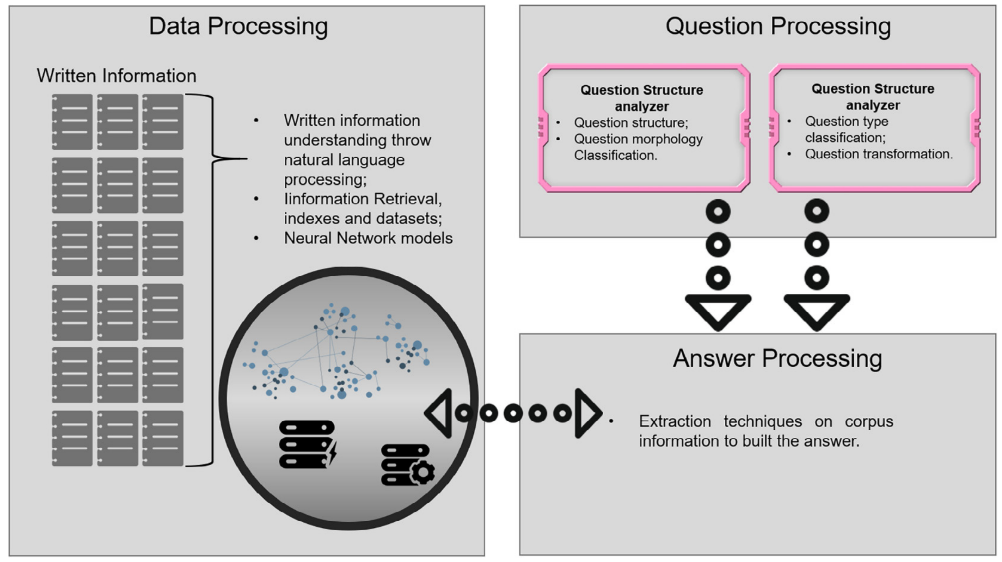
\includegraphics[width=1\linewidth]{images/arch.png}
    \caption[Allgemeine Systemarchitektur mit 3 Hauptmodulen]{Allgemeine Systemarchitektur mit 3 Hauptmodulen \cite [S. 3]{CalijorneSoares2018ASystems}}
    \label{fig:architektur}
\end{figure}
\section{Geschichte des Question Answerings}

%%%%%%%%%%%%%%%%%%%%%%%%%%%%%%%%%%%%%%%%%%%%%%%%%%%%%%%%%%%%%%%%%%%%%%    
% TODO
%    %graphs []
%
%%%%%%%%%%%%%%%%%%%%%%%%%%%%%%%%%%%%%%%%%%%%%%%%%%%%%%%%%%%%%%%%%%%%%%    

Tatsächlich geht die Geschichte des Question Answering bis in die 60'er Jahre zuruck. Mit \citep{Simmons1964IndexingQuestions} wurde im Jahr 1965 versucht, englische Fragen mittels eines Computers zu beantworten. Mit \textbf{BASEBALL} \citep{Green1961Baseball:Question-answerer} wurden bereits im Jahr 1961 Baseball-Spiele analysiert. Während BASEBALL selbst nach aktuellen Maßstäben im Umgang mit der Syntax und Semantik von Fragen relativ hoch entwickelt war, war es in Bezug auf seine Domäne - nur Baseball - und durch die Tatsache, dass es in erster Linie als Schnittstelle zu einer strukturierten Datenbank gedacht war, begrenzt und nicht als Schnittstelle zu einer großen Textsammlung gedacht. In dieser Hinsicht war BASEBALL als „Frontends für Datenbanken in natürlicher Sprache“ konzipiert wurden. Anstatt Benutzer dazu zu zwingen, die Struktur einer Datenbank und eine spezielle Sprache für deren Abfrage zu lernen, bestand das Ziel darin, die Kommunikation in ihrer eigenen Sprache mit einer Schnittstelle zu ermöglichen. Das Frontend konnte dann die Sprache verstehen und diese in eine Datenbankabfrage umwandeln \citep[S. 279-280]{Hirschman2001NaturalHere}.

Das bekannteste andere frühe Werk in dieser Tradition ist das \textbf{LUNAR}-System. LUNAR wurde entwickelt, \enquote{um einem Mondgeologen einen bequemen Zugriff auf die chemischen Analysedaten zur Mondgesteins- und Bodenzusammensetzung zu ermöglichen, diese zu vergleichen und auszuwerten, die sich infolge der Apollo-Mondmission angesammelt haben} \citep{4-8ProgressGeology} . LUNAR könnte Fragen beantworten wie \enquote{Wie hoch ist die durchschnittliche Aluminiumkonzentration in Gesteinen mit hohem Alkaligehalt?} oder \enquote{Wie viele Brescias enthalten Olivin?}. Es war mehr als ein Spielzeug und wurde 1971 auf einer Mondwissenschaftskonvention demonstriert und konnte 90\% der von arbeitenden Geologen gestellten Fragen ohne vorherige Anweisung zur Formulierung beantworten \citep[S. 280]{Hirschman2001NaturalHere}. 


In den 1980er und 1990er Jahren wurden Wissensbasierte Systeme, die normalerweise nur für beschränkte Anwendungsbereiche entwickelt wurden, sehr beliebt. Wissensbasierte Systeme  eignen sich gut für ein Framework zur Beantwortung von Fragen, bei dem der Benutzer mit einem bestimmten Problem konfrontiert wird. Der Zugriff auf die Wissensdatenbank erfolgt normalerweise über Menüs oder eine Schnittstelle in natürlicher Sprache. Das System selbst stellt dem Benutzer interaktiv zusätzliche Fragen, um die Absicht des Benutzers besser zu verstehen. Um das Problem zu lösen, verwendet das System das in der Wissensdatenbank verfügbare Wissen und die vom Benutzer bereitgestellten zusätzlichen Informationen \citep [S. 5415]{Kolomiyets2011APerspective}. Bekannte Beispiele sind das \textbf{MYCIN-System} \citep{edward1976shortliffe}, welches als Enzyklopädie fpr medizinische Konzepte Antworten geben sollte und das \textbf{SHRDLU-System} \citep{winograd1971procedures} welches durch sein Sprachverständnis Roboter steurte und somit Spielzeugblöcke bewegen konnte.

Die Ära des zeitgenössischen Question Answerings begann 1999 mit der aufnahme des Question Answerings in das Wettbewerbspfad von \textbf{TREC-9} (\enquote{The ninth Text REtrieval Conference}), welches eine  Konferez ist, die die Forschung für das Information Retrieval fördern soll. In dieser Konforenz wurde eine Herausforderung für das Question Answering definiert, welches darin bestand, angesichts einer großen Sammlung von Textdokumenten eine präzise Antwort auf eine Frage in natürlicher Sprache zu geben \citep{VoorheesReportTREC-9}. TREC hatte einen großen Einfluss auf das Interesse am Question Answering und auf die Entwicklung von Bewertungsmaßnahmen, mit denen die Leistung von Systemen verglichen wird \citep{voorhees2005trec}. 


\section{Klassifizierung der QA-Systeme}
\subsection{Klassifizierung nach der Domäne}
%%%%%%%%%%%%%%%%%%%%%%%%%%%%%%%%%%%%%%%%%%%%%%%%%%%%%%%%%%%%%%%%%%%%%%    
% TODO
%   % Tabelle mit den Arten
%%%%%%%%%%%%%%%%%%%%%%%%%%%%%%%%%%%%%%%%%%%%%%%%%%%%%%%%%%%%%%%%%%%%%%    
Im Allgemeinen kann das Question Answering in Open-Domain Question Answering und Closed-Domain Question Answering unterteilt werden. Die Beantwortung von Fragen zu geschlossenen Domänen befasst sich mit Fragen unter einer bestimmten Domäne und kann als einfachere Aufgabe angesehen werden, da NLP-Systeme domänenspezifisches Wissen nutzen können, das häufig in Ontologien formalisiert wird. Alternativ kann sich eine geschlossene Domäne auf eine Situation beziehen, in der nur eine begrenzte Art von Fragen akzeptiert wird, z. B. Fragen, die eher beschreibende als prozedurale Informationen erfordern. Die Beantwortung von Fragen in offenen Domänen behandelt Fragen zu fast allem und kann sich nur auf allgemeine Ontologien wie \enquote{DBpedia} stützen \citep{Mervin2013AnSystem}. Einen Vergleich der Systeme kann aus der Tabelle \ref{tab:tab1} entnommen werden.

\textbf{Open Domain Question Answering} Systeme sind nicht auf eine bestimmte Domain beschränkt und bieten eine kurze Antwort auf eine Frage in natürlicher Sprache. Das Web ist die beste Quelle, um Informationen zu erhalten, da das Internet in großem Umfang genutzt wird, und die meisten webbasierten Systeme zur Beantwortung von Fragen funktionieren für offene Domänen \citep{yogish2016survey}. Das Open-Domain-QS-System hängt von Informationen wie dem World Wide Web und der universellen Ontologie ab und kann fast alles mit beantworten \citep{SreelakshmiOPENLABELING}. Open Domain QA-Systeme wenden ein allgemeines Vokabular an und erfordern kein domänenspezifisches Vokabular. Benutzer benötigen keine domänenspezifischen Kenntnisse, um Fragen vorzubereiten. Open Domain QA-Systeme bestehen aus einem großen \enquote{Repository} von Fragen und suchen im Allgemeinen nach Antworten in einer großen Dokumentensammlung. In Open Domain QA-Systemen kann Wikipedia als Informationsquelle verwendet werden. In Open-Domain QA-Systemen ist die Qualität der Antworten, die von Benutzern generiert werden, gering. Open Domain QA-Systeme sind domänenunabhängig und hängen von Weltdaten und der grundlegenden Ontologie ab \citep{biswas2014framework}. Im Open Domain QA-System gibt es keine Einschränkung der Domain. Open-Domain QA-Systeme eignen sich eher für eine große Anzahl von Gelegenheitsbenutzern \citep[S. 20]{ChandraASystem}.

In \textbf{Closed Domain Question Answering} Systemen gibt es eine Einschränkung der Domäne, die beantwortung der Fragen ist verbunden an eine bestimmte Domäne. Das System besteht aus einem begrenzten \enquote{Repository} domänenspezifischer Fragen und kann eine begrenzte Anzahl von Fragen beantworten. Daher ist in QA-Systemen mit geschlossenen Domänen die Qualität der Antworten hoch. QA-Systeme für geschlossene Domänen beantworten domänenspezifische Fragen, und Antworten werden in domänenspezifischen Dokumentensammlungen gesucht. QA-Systeme mit geschlossenen Domänen sind so konzipiert, dass sie Antworten aus strukturierten Daten (z. B. Datenbanken), unstrukturierten Daten (Freitexte) und halbstrukturierten Daten (z. B. XML-kommentierten Texten) erhalten. QA-Systeme für geschlossene Domänen verwenden domänenspezifische Terminologie und Ontologie. In der Literatur wurden verschiedene QA-Systeme für geschlossene Domänen entwickelt, z Domänen-QA-Systeme. QA-Systeme mit geschlossener Domäne mit begrenzter Arbeitsdomäne sind nützlicher für Benutzer mit Domänenexperten, die spezielle Antworten benötigen \citep[S. 20]{ChandraASystem}.

\begin{table}[H]
{\small
    \begin{tabularx}{\textwidth}{X|X|X} 
    
                  &\textbf{Open Domain QA}  & \textbf{Closed Domain QA}  \\ 
\hline    
    \textbf{Domäne}      & unbeschränkt        & beschränkt         \\ 
    \textbf{Quelle}   & Web        & Datenbanken          \\ 
    \textbf{Qualität} & gering        & gut           \\ 
    \textbf{Nutzer} & Gelegenheitsnutzer        & Domänenexperten           \\ 
    \end{tabularx}
\caption{Vergleich des Open-Domain und Closed-Domain Question Answerings}
    \label{tab:tab1}
}
\end{table}


\subsection{Klassifizierung nach dem Fragetyp}

Neben der Domäne, werdem Question Answering Systeme nach Fragetypen klassifiziert. Diese Fragentypen sind \citep[S. 20-21]{ChandraASystem}:

\begin{itemize}
    \item \textbf{Faktoide Fragen} 
    Die faktoiden Fragen beginnen gewöhnlich mit einem W-Wort (\enquote{Was?}, \enquote{Wann?}, \enquote{Wer?}, \enquote{Wie?}). Diese Fragen sind einfach zu beantworten und basieren auf Fakten. Sie müssen in einem einzigen Satz oder einer kurzen Phrase beantwortet werden. Zum Beispiel die faktoide Frage \enquote{Was ist die Hauptstadt von Indien?} fragt nach einem Städtenamen und es ist einfach. Die Antworttypen für faktoide Fragen werden im Allgemeinen als Entitäten bezeichnet \citep{khillare2014comparative}. Fragen vom Typ Faktoid ergeben eine zufriedenstellende Antwortleistung. Im Allgemeinen sind Fragen vom Typ Faktoid ein großes Repository von Fragen. Fragen vom Typ Faktoid erfordern keine komplexe Verarbeitung natürlicher Sprache, um Antworten zu erhalten. Die Identifizierung von Fragen vom Typ Faktoid und ihre Unterklassifizierung ist eines der Forschungsprobleme im Fragebeantwortungssystem. Fragen vom Typ Faktoid können mit kurzen Sätzen wie Organisationen, Personen, Daten und Orten beantwortet werden.
    \item \textbf{Listen Fragen}
    Die Fragen nach Listen benötigen eine Liste von Fakten oder Entitäten als Antworten, z.B, listen sie die Namen der Filme im Jahr 2017 auf. Bei diesen Fragen werden die Antworttypen als Entitäten bezeichnet. Daher können die Antworten auf Listenfragen eine gute Genauigkeit ergeben. QA-Systeme die solche Fragen beantworten benötigen keine tiefgreifende Verarbeitung natürlicher Sprache, um Antworten abzurufen. Die Techniken, die bei Fragen vom Typ Faktoid angewendet werden, eignen sich gut für Fragen vom Listentyp \citep{wu2015leveraging}.
    \item \textbf{Bestätigungsfragen} 
    Bestätigungsfragen benötigen Antworten in Form von \enquote{Ja} oder \enquote{Nein}. Zum Beispiel die Bestätigungsfrage "Ist Jesus Christus Gott und Mensch?", fragt nach der Antwort Ja oder Nein. Zur Beantwortung von Bestätigungsfragen sind Weltwissen, Inferenzmechanismen und logisches Denken erforderlich. Einer der Vorteile von Fragen vom Typ Bestätigung, die in QA-Systemen gestellt werden, besteht darin, dass einige erfahrene Benutzer möglicherweise nach Informationen suchen möchten, die für neues Wissen logisches Denken und Weltwissen erfordern \citep{tanwar2014effective}. Die Nachteile von Bestätigungsfragen, die in QA-Systemen gestellt werden, bestehen darin, dass sie ein höheres Maß an Techniken zum Erwerb und Abrufen von Wissen benötigen. Abgesehen von den oben genannten Fragen zum Bestätigungstyp können Meinungsfragen erforderlich sein. QA-Systeme verwenden Social Web- und Opinion Mining-Techniken, um Antworten auf die Fragen vom Typ \enquote{Meinung} zu erhalten. Die Vorteile von Meinungsfragen sind, dass Meinungsdatenquellen öffentliche Meinungen enthalten, die den Benutzern bei der Beurteilung der Produkte helfen können. Die Nachteile von Fragen vom Typ Meinung sind die Erkennung von Spam oder gefälschten Inhalten in Textsystemen, was zu Problemen beim echten Argument-Mining des Textes führt.
    \item \textbf{Kausale Fragen} 
    Die Antworten auf kausale Fragen werden \enquote{nicht als faktoide Fragen} bezeichnet. Kausale Fragen benötigen Antworten auf Beschreibungen einer Entität und können mit \enquote{Warum?} oder \enquote{Wie?} beantwortet werden. Kausale Fragen werden von Benutzern gestellt, die Antworten als Gründe, Erklärungen, Ausarbeitungen usw. in Bezug auf bestimmte Objekte oder Ereignisse wünschen.
    z. B. Warum hält Professor Y eine Rede im Auditorium?
    \item \textbf{Hypothetische Fragen}
    Bei hypothetischen Fragen werden Informationen angefordert, die sich auf ein hypothetisches Ereignis beziehen und nicht spezifisch sind. Hypothetische Fragen beginnen normalerweise mit \enquote{Was würde passieren, wenn?}. Die Zuverlässigkeit und Genauigkeit dieser Fragen ist gering und hängt von den Benutzern und dem Kontext ab.
    \item \textbf{Komplexe Fragen}
    Um komplexe Fragen wie \enquote{Was sind die Gründe für Luftverschmutzung?} beantworten zu können, müssen oft Informationen aus mehreren Dokumenten ableiten und synthetisieren werden. Zur Beantwortung komplexer Fragen sind komplexe Verfahren erforderlich. Komplexe Fragen erfordern mehrere unterschiedliche Arten von Informationen, und es ist schwierig, Antworten zu finden. Nach \citep{basuki2016statistical} besteht eine komplexe Frage aus mehreren unabhängigen Fragen, und jede Frage sucht nach einer Antwort aus mehreren Dokumenten.
    
\end{itemize}


\subsection{Klassifizierung nach der Datenquelle}
Neben der Hauptarchitektur können QA-Systeme nach der herkunft Ihrer Daten klassifiziert werden. In \citep{Jurafsky2014SpeechProcessing} wird das QA unterteilt in Information Retrieval QA,  wissensbasiertes QA und hybrides QA \citep{Ojokoh2019ASystems}:


%%%%%%%%%%%%%%%%%%%%%%%%%%%%%%%%%%%%%%%%%%%%%%%%%%%%%%%%%%%%%%%%%%%%%%
%n-gram pattern extraction -- NLP!!
%%%%%%%%%%%%%%%%%%%%%%%%%%%%%%%%%%%%%%%%%%%%%%%%%%%%%%%%%%%%%%%%%%%%%%

\begin{itemize}
    \item \textbf{Information Retrieval QA} Basiert auf einer sehr großen Menge von Informationen, die im Web als Text oder in Ontologien vorhanden sind. Diese Art von QA bietet eine Antwort auf die Fragen des Benutzers indem es Textausschnitten aus dem Web oder Korpora abruft. Eine faktoide Abfrage lautet z.B.: \enquote{Wer ist der Präsident von Nigeria?}. Die Antwort lautet \enquote{Präsident Buhari im Urlaub in London}. IR-Methoden extrahieren Passagen direkt aus den passenden Dokumenten, welches sie von der gestellten Frage ableiten. Zunächst verarbeitet diese Methode die Abfrage vor, um den Antworttyp (Person, Ort oder Zeit) zu ermitteln. Die Genauigkeit der Fragenklassifizierung ist für faktoide Fragen mit benannten Entitäten als erwartete Ausgabe relativ hoch, aber Fragetypen wie Bestätigungsfragen, kausale Fragen, hypothetische Fragen oder komplexe Fragen können viel schwieriger sein, da sie ein tiefes Verständnis der Abfrage erfordern. Anschließend werden Abfragen für die Suche erstellt, um Suchmaschinen abzufragen. Dies beinhaltet das Isolieren von Begriffen aus der Frage, die eine Abfrage bilden, die dann an ein Abrufsystem gestellt werden. Dies beinhaltet gelegentlich das Entfernen von Stoppwörtern und Satzzeichen. Als nächstes müssen die von der Suchmaschine gelieferten Dokumente oder Passagen geordnet werden. Dieses Ordnen der Dokumente kann z.B. mit der Methode \enquote{tf-idf}, einer Relevanzmodellierungsansatz für die Bewertung von Passagen oder Dokumenten ausgeführt werden \citep[S. 467 - 470]{Jurafsky2014SpeechProcessing}.
    Zuletzt werden potenzielle Zeichenfolgen für die Extraktion bestimmt. Dabei können z.B.: Methoden wie \enquote{pattern extraction} \citep{soubbotin2001patterns} oder \enquote{n-gram} \citep{brill2001data} verwendet werden.
    \item \textbf{Wissensbasiertes QA} Beliebte Ontologien wie DBpedia \citep{bizer2009dbpedia} oder Freebase \citep{bollacker2008freebase} enthalten Subjekt-Prädikat-Objekt-Tripel, die aus Wikipedia-Infoboxen und den strukturierten Daten aus Wiki-Artikeln extrahiert wurden. 
    
    Bei der wissensbasierten QA-Systemen werden Antworten auf Fragen in natürlicher Sprache gegeben, indem sie einer Abfrage über eine Ontologie zugeordnet werden. Welche logische Form auch immer aus der Zuordnung abgeleitet wird, wird zum Abrufen von Fakten aus Datenbanken verwendet. Die Datenquelle kann eine beliebige komplexe Struktur sein, z. B. wissenschaftliche Fakten oder räumliche Messwerte, für die komplexe logische oder SQL-Abfragen erforderlich wären. Es können auch Tripel sein, die in einer Datenbank, Freebase oder DBpedia zusammengesetz wurden \citep[S. 476]{Jurafsky2014SpeechProcessing}. Das Zuordnen einer vom Benutzer gestellten Abfrage zu einer logischen Form wird von semantischen Parsern durchgeführt \citep{hoffner2017survey}. Um die Zuordnung vom Text (Frage in natürlicher Sprache) zu einer logischen Abrage durchzuführen, verwendet die KB-QA-Systeme einige dieser Methoden \citep[S. 477 - 479]{Jurafsky2014SpeechProcessing}: 
    \begin{itemize}
        \item \textbf{Regelbasierte Methoden:} Diese Methoden konzentrieren sich auf die Entwicklung manuell erstellter Regeln, um häufig vorkommende Assoziationen aus der Abfrage zu extrahieren \citep{ravichandran2002learning}.
        \item \textbf{Überwachte Methoden:} Dazu werden Trainingsdaten verwendet, die Fragenpaare und ihre logischen Formen enthalten, und anschließend ein Modell erstellt, welches die Fragen seiner logischen Form zuordnet \citep{tirpude2015closed}.
        \item \textbf{Semi-Überwachte Methoden:} 
        Es gibt noch keine Datensätze, die alle möglichen Fragenformen, die in den Abfragen vorliegen können, beinhalten. Aus diesem Grund wird die Textredundanz von den meisten Methoden genutzt, um Abfragen zu Beziehungen oder anderen Wissensstrukturen zuzuordnen. Diese Methode wird von IBM Watson \citep{high2012era} und den meisten hybriden QA-Systemen. 
    \end{itemize}
    \item \textbf{Hybrides QA}  Beinhaltet die Verwendung strukturierter Wissensdatenbanken und Textdatensätze in hybrider Form. Das DeepQA-System \citep{ferrucci2010building} ist ein hybrides QA-System, das nicht nur auf einer Informationsquelle basiert. Dieses System extrahiert eine Vielzahl von Quellen, benannte Entitäten, Analysen, Beziehungen, ontologische Informationen und ruft dann  Wissensdatenbanken für Kandidatenantworten ab. Die Bewertung wird dann für jede Kandidatenantwort unter Verwendung einer Reihe von Wissensdatenbanken wie zeitliches Denken, Geodatenbanken und taxonomische Klassifizierung durchgeführt \citep[S. 479 - 483]{Jurafsky2014SpeechProcessing}.
\end{itemize}








\section{Methoden und Algorithmen}
In \citep [S. 5418 - 5427]{Kolomiyets2011APerspective} werden die wichtigsten Methoden für das Question Answering vorgestellt. Eine Auswahl dieser Methoden wird in diesem Abschnitt beschrieben:
\subsection{Bag-of-words}

    
Ein Textdokument wird so dargestellt, als wäre es eine Wortsammlung, d.h. eine ungeordnete Reihe von Wörtern, deren Position ignoriert wird, wobei nur ihre Häufigkeit im Dokument relevant ist \citep [S. 58]{Jurafsky2014SpeechProcessing}. 
Bag-of words ist der einfachste Fall, wenn Abfragen und in einem \enquote{Wortbeutel} dargestellt werden.
Es wird das sog. Boolesches Modell verwendet, bei dem der aus der Abfrage erstellte Boolesche Ausdruck mit der Dokumentdarstellung übereinstimmen muss. Beim BoW werden die Sätze in ihre Tokens zerlegt und nach ihrer Häufigkeit im Satz gezählt. Im folgenden Beispiel gibt es eine Abfrage und ein Dokument, welches als Kandidat für die Antwort gelten soll. Das BoW-Verfahren, kann dafür benutzt werden, einen Abgleich der Wörter zwischen der Abfrage und dem Dokument zu machen. Es ist zu sehen, wenn man die Stoppwörter \enquote{ist} und \enquote{die} herausnimmt, dass Paris mit einer Häufigkeit von 2 im Kandidaten Dokument auftaucht und somit als Antwort angenommen werden kann:

\begin{verbatim}
Abfrage = ["Was ist die Hauptstadt von Frankreich?"]

Dokument = ["Paris ist die Hauptstadt und als Agglomeration 
mit dem Gemeindeverband Métropole du Grand Paris und den 
umliegenden Gebieten der  Region Île-de-France..."]

BoW = {'ist': 2, 'die': 2, 'hauptstadt': 2, 'paris': 2, 'und': 2, 
'was': 1, 'von': 1, 'frankreich': 1, 'als': 1, 'agglomeration': 1, 
'mit': 1, 'dem': 1, 'gemeindeverband': 1, 'métropole': 1, 'du': 1, 
'grand': 1, 'den': 1, 'umliegenden': 1, 'gebieten': 1, 'der': 1, 
'region': 1, 'île': 1, 'de': 1, 'france': 1}
\end{verbatim}

Das BoW kann dafür benutzt werden, die Abfrage, eine Frage die in das QA-System gestellt wird, mit einem Dokument oder einer Passage zu matchen, wie in Abbildung \ref{fig:bow} zu sehen ist: 


\begin{figure}[H]
\centering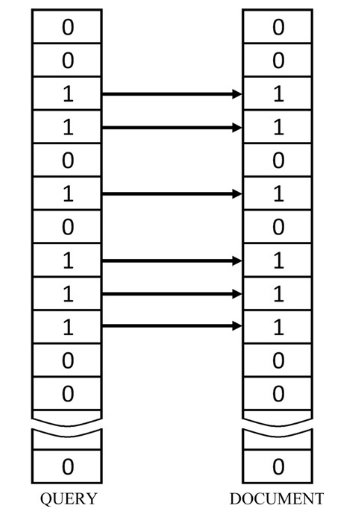
\includegraphics[width=0.3\linewidth]{images/bow.png}
\caption[Übereinstimmung von Abfrage und Dokumenten mit BoW]{Übereinstimmung von Abfrage und Dokumenten mit BoW \cite [S. 5419]{Kolomiyets2011APerspective}}
\label{fig:bow}
\end{figure}

Bei der Analyse der Frage und auch bei der Analyse von Dokumenten und Sätzen, ist der BoW-Ansatz ein sehr einfacher Ansatz, welches die strukturellen Beziehungen zwischen Wörtern ignoriert. Die abgerufenen Informationen sind möglicherweise nicht sehr genau. Beispiel: Für die Abfrage \enquote{Ein Kind mit braunen Haaren, das einen gelben Pullover mit Blue Jeans trägt}, wird möglicherweise ein ein Abruf gemacht, welches ein Mädchen mit gelben Hosen und einem blauen Pullover zeigt, da nur die Häufigkeit der Wörter und nicht die Struktur berücksichtigt wird \citep [S. 5419]{Kolomiyets2011APerspective}. Obwohl diese Modelle in der Information Retrival und Suchtechnologie sehr beliebt sind, fehlt ihnen typischerweise die Präzision, die für die Beantwortung von Fragen erforderlich ist, selbst für die Beantwortung einfacher Sachfragen, die das Abrufen einer Entität erfordern (z. B. Name der Person, Datum) \citep{moldovan2003performance}. Beim  herkömmlichen Question Answerring hat sich das BoW jedoch als nützlich für die anfängliche grobe Filterung von Dokumenten und Sätzen erwiesen, die offensichtlich keine Relevanz für die vorliegende Informationsfrage haben. Es hat sich gezeigt, dass korrekte Antworten mit einer begrenzten Anzahl von Zuordnungsregeln zu den Abfragen gefunden werden können, indem die Redundanz der verfügbaren Antworten ausgenutzt wird \citep{brill2001data}.

    
    
\subsection{Morphosyntaktische Analyse von Aussagen in natürlicher Sprache}

In einer morphologischen Analyse können Stemming und Lemmatisierung nützlich sein, da sie die Chancen verbessern, eine gute Übereinstimmung der Abfrage mit einem Antwortsatz zu finden. Stemming normalisiert Wörter zu ihrer gemeinsamen Wurzelform. Zum Beispiel beziehen sich Katze und Katzen auf denselben Stamm - Katze. Im Gegensatz dazu identifiziert die Lemmatisierung das Lexem, also die Bedeuting \citep[S. 5419]{Kolomiyets2011APerspective}. Diese Operationen reduzieren jedoch die in einem Begriff enthaltenen Informationen. In vielen Sprachen definieren Flexionsformen von Substantiven und Pronomen, die syntaktische oder semantische Funktion einer Phrase, eines Satzes oder eines Satzbestandteils (z. B. Identifizierung von Subjekt-, Objekt- oder Indizien) \citep{nivre2006maltparser}. Der einfachste Ansatz zur Erkennung der Satzstruktur ist duch der Ansatz mit dem n-Gramm Verfahren \citep{brill2002analysis}, jedoch gibt es für eine Syntaktische Analyse einer Abfrage viele verschiedene NLP Methoden, wie das \enquote{part-of-speech} (POS) Verfahren, um die Nomen von den Verben zu unterscheiden und das \enquote{phrase chunking} um Idiomatische Ausdrücke zu finden \citep[S. 5419]{Kolomiyets2011APerspective}. Zusätzlich kann durch das Aufteilen eines Satzes in seine Bestandteile und das finden der Abhängigkeiten ein Abhängigkeitsbaum erstellt werden \citep{cui2005question}.  

\begin{figure}[H]
\centering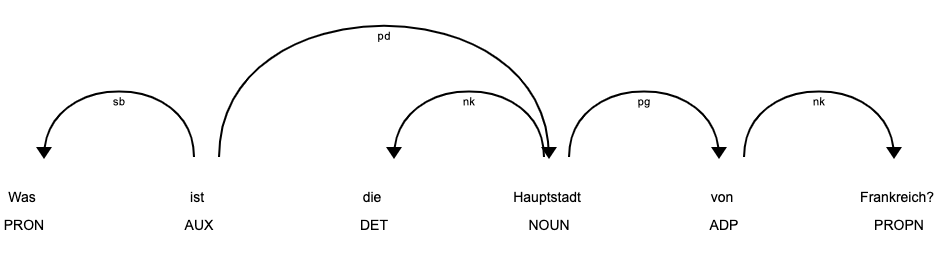
\includegraphics[width=0.9\linewidth]{images/dep.png}
\caption[Dependenzstruktur einer Frage]{Dependenzstruktur einer Abfrage}
\label{fig:dep}
\end{figure}

In Abbildung \ref{fig:dep} wird ein Beispiel für eine Analyse einer Abfrage, nach den Abhängigkeiten der einzelnen Elemente der Abfrage untereinander abgebildet. Der Token \enquote{Hauptstadt} hat zum Token \enquote{die} und \enquote{von} eine Abhängigkeit. Ebenso ist eine Abhängigkeit zwischen den Tokens \enquote{ist} und \enquote{Hauptstadt} festzustellen.

Die morphosyntaktische Analyse natürlicher Sprachausdrücke führt zu einer besseren Erfassung der strukturellen Beziehungen zwischen
Wörtern in einem Satz oder einer Frage, was zu einer angereicherten Bedeutungsdarstellung führt \citep[S. 5420]{Kolomiyets2011APerspective}. Die Abhängigkeit von morphosyntaktischen Mustern wurde erfolgreich für die automatische Generierung von Multiple-Choice-Fragen aus Texten nachgewiesen \citep{mitkov2006computer}, ihr Potenzial kann jedoch auf die allgemeine Beantwortung von Fragen ausgeweitet werden \citep[S. 5420]{Kolomiyets2011APerspective}.

\subsection{Semantische Klassifikation des erwarteten Antworttyps}
In Abbildung \ref{fig:lir} ist die Verteilung von 1.000 TREC-Fragen auf die Fragenhierarchie abgebildet. \enquote{Grobe Klassen} sind fett gedruckt und werden von ihren Verfeinerungen in feine Klassen gefolgt. \enquote{\#} ist die Anzahl der Fragen in jeder Klasse. Die Fragen wurden von \citep{li2006learning} manuell klassifiziert.
\begin{figure}[H]
\centering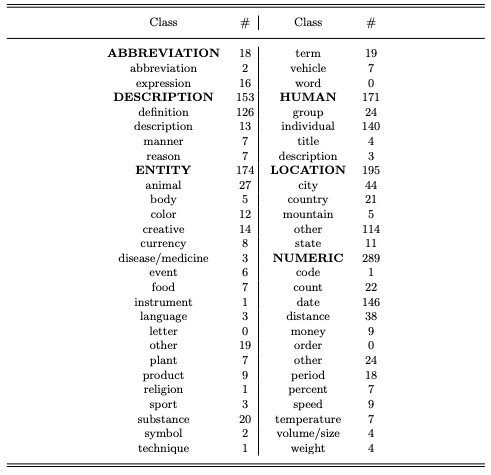
\includegraphics[width=0.7\linewidth]{images/lir.png}
\caption[Klassifikation von faktoiden Fragen]{Klassifikation von faktoiden Fragen \citep{li2006learning}}
\label{fig:lir}
\end{figure}



Eine Frage oder Anweisung in natürlicher Sprache gibt zusätzliche Informationen über die Art der Informationen, die als Antwort erwartet wird. Zum Beispiel ist die Suche möglicherweise nach einer Person, dem Namen eines Unternehmens, dem Ort, dem Datum oder sogar einem Bild einer Person in einem Video von Interesse. Bei der Beantwortung von Fragen ist es üblich geworden, die semantische Klasse der erwarteten Antwort in der Frage und die entsprechende semantische Klasse des Antwortkandidaten in der Informationsquelle automatisch zu identifizieren. Bei faktoiden Fragen entsprechen die Fragetypklassen einem erwarteten Antworttyp, die in Taxonomien oder Frage-Ontologien gespeichert werden \citep[S. 5420]{Kolomiyets2011APerspective}. 
Die bekannteste Taxonomie für erwartete Antworttypen in Bezug auf faktoide Fragen ist die von \citep{li2006learning}, welches aus sechs Kategorien und fünfzig feinen Kategorien (z. B. Abkürzung, Beschreibung, Entität, Mensch, Ort und Numerisch, Farbe, Stadt usw.) besteht.

In jüngerer Zeit wurden überwachte Techniken des maschinellen Lernens populär, die ein Klassifizierungsmodell anhand von Beispielen trainieren. Diese Modelle werden manuell kommentiert (Fragen mit den entsprechenden Antworttypen). Das Erstellen eines Trainingssets ist ein zeitaufwändiger Prozess, erfordert jedoch keine Regeln, die festgelegt werden müssen. Die Klassifizierung einer neuen Frage basiert einfach auf den Mustern, die aus dem Trainingssatz gelernt wurden. Es kann zwischen einer großen Anzahl von Techniken ausgewählt werden, um Fragen zu Klassifizieren \citep[S. 5421]{Kolomiyets2011APerspective}. In \citep{zhang2003question} wird das SVM-Verfahren angewendet und es wird gezeigt, dass das SVM die anderen Methoden des machinellen Lernens zur Fragenklassifizierung übertroffen hat.

Das Ermitteln des erwarteten Antworttyps hängt stark mit realen Fragen zusammen, während Fragen in natürlicher Sprache häufig in anderen Formen gestellt werden. Die Abfrage \enquote{Zeige mir ein Kind mit braunen Haaren, das einen gelben Pullover mit Blue Jeans trägt} ist eine komplexe (Ab)-frage oder Abfrageanweisungen. Solche Abfragen   haben häufig viele zusätzliche Einschränkungen, die einen feineren Informationsbedarf ausweisen. Welche Art von Informationen wichtiger ist als andere, kann somit nicht vollständig ermittelt werden \citep[S. 5422]{Kolomiyets2011APerspective}. 
\subsection{BERT-basiertes Question Answering}


\section{Bewertung von Question Answering Systemen}
\textbf{\enquote{Precision}} und \textbf{\enquote{Recall}} sind die traditionellen Maße, die für das Information Retrievalals Metrik verwendet werden, während das \textbf{\enquote{F-Maß}} das harmonische Mittel für Precision und Recall ist. Diese drei Metriken sind gegeben durch:

\begin{xequation-} 
\centering ${Precision}= \frac{\text{Anzahl der richtigen Antworten}}{\text{Anzahl der beantworteten Fragen}}$
\caption[Precision]{Precision} 
    \label{eqn:PRE}
\end{xequation-} 

\begin{xequation-} 
\centering ${Recall}= \frac{\text{Anzahl der richtigen Antworten}}{\text{Anzahl der zu beantwortenden Fragen}}$
\caption[Recall]{Recall} 
    \label{eqn:REC}
\end{xequation-} 

\begin{xequation-} 
\centering ${F_1}= 2 \cdot \frac{\text{Precision} \cdot \text{Recall}}{\text{Precision} + \text{Recall}}$
\caption[F-Maß]{F-Maß} 
    \label{eqn:FME}
\end{xequation-} 




Eine übliche Bewertungsmetrik für die Beantwortung faktoider Fragen, ist der \textbf{\enquote{Mean Reciprocal Rank} (MRR)}, welches 1999 in den TREC \citep{voorhees1999proceedings} aufgenommen wurde. MRR setzt einen Testsatz von MRR-Fragen voraus, die mit korrekten Antworten vom Menschen gelabelt wurden. MRR geht auch davon aus, dass Systeme eine kurze Liste von Antworten oder Passagen zurückgeben, welches die Antworten enthalten. Jede Frage wird dann nach dem Kehrwert des Ranges der ersten richtigen Antwort bewertet. Wenn das System beispielsweise fünf Antworten zurück gibt, die ersten drei jedoch falsch sind und daher die am höchsten eingestufte richtige Antwort an vierter Stelle steht, beträgt die gegenseitige Rangbewertung für diese Frage 1/4. Fragen die keine korrekten Antworten enthalten, werden mit Null bewertet. Die Punktzahl eines Systems ist dann der Durchschnitt der Punktzahl für jede Frage im bewerteten Satz. Die Bewertung eines Systems mit MRR, dass einen Satz von Antworten für einen Testsatz zurückgibt und welches aus N Fragen besteht, wird folgendermaßen definiert \citep [S. 483]{Jurafsky2014SpeechProcessing}:

\begin{xequation-} 
\centering ${MRR}= \frac{1}{n} \sum_{i=1}^{n} \frac{1}{\text{rank}_i}$
\caption[Mean Reciprocal Rank (MRR)]{Mean Reciprocal Rank (MRR)} 
    \label{eqn:MRR}
\end{xequation-} 

Angenommen dem Question Answering werden 3 Fragen gestellt. Das QA-System gibt hat nun 3 Vorschläge als Antwort dieser Frage abgegeben. Die erste Frage wurde beim dritten Versuch richtig beantwortet. Somit beträgt der \enquote{Reciprocal Rank} für diese Frage 1/3. Wenn diese Frage beim ersten Treffer beantwortet wurde, würde der \enquote{Reciprocal Rank} 1 ergeben. Der MRR ist also der Mittelwert der ermittelten \enquote{Reciprocal Ranks}.







%%%%%%%%%%%%%%%%%%%%%%%%%%%%%%%%%%%%%%%%%%%%%%%%%%%%%%%%%%%%%%%%%%%%%%
\chapter{Technologien und Werkzeuge}
%%%%%%%%%%%%%%%%%%%%%%%%%%%%%%%%%%%%%%%%%%%%%%%%%%%%%%%%%%%%%%%%%%%%%%

%%%%%%%%%%%%%%%%%%%%%%%%%%%%%%%%%%%%%%%%%%%%%%%%%%%%%%%%%%%%%%%%%%%%%%
%4 Seiten
%%%%%%%%%%%%%%%%%%%%%%%%%%%%%%%%%%%%%%%%%%%%%%%%%%%%%%%%%%%%%%%%%%%%%%
Die im folgenden Kapitel beschriebenen Technologien und Tools werden für die Entwicklung des QA-Chatbot-Prototyps verwendet. Die Beschreibung ist nur oberflächlich. Detaillierte Informationen zur verwendeten Software, zur Systemumgebung und zu den einzelnen installierten Paketen befinden sich in den Anhängen 4 und 5. %todo where
\section{Python}
Python ist eine von der Python Software Foundation weiterentwickelte und veröffentlichte Programmiersprache, die sowohl als objektorientierte Programmiersprache als auch als Skriptsprache angesehen werden kann. Python benötigt relativ wenige Schlüsselwörter, zeichnet sich durch seine Einfachheit, Klarheit und Erweiterbarkeit aus und verfügt über eine große Anzahl wissenschaftlicher Programmbibliotheken auf dem Gebiet Data-Science und wird daher immer mehr zum zentralen Werkzeug. 
Durch so genannte virtuelle Umgebungen, lassen sich die Entwicklungen mittels Python gezielt auf eine Python Version begrenzen und nur bestimmte Pakete mit installieren lassen, somit kann man eine Umgebung für die Softwareverteilung verwenden \citep[S. 2]{GrotzGrundkurs0.1.2d}.
\section{Spacy}
Spacy ist ein Python-Module für die NLP-Entwicklung. Der Fokus liegt dabei auf Geschwindigkeit und Einfachheit. Dabei liefert Spacy die essentiellen NLP-Aufgaben und für jede Aufgabe ist genau ein Algorithmus implementiert worden. Es werden neben Englisch auch Deutsch, Spanisch und Französisch angeboten. Die Annotationen werden dabei in dem Objekt \enquote{doc} gespeichert. Einzelne Wörter werden dabei zu Tokens gemacht. Die Sätze werden automatisch gesplittet und Spacy liefert daneben die Möglichkeit, Named Entity Recognition, den Sentiment, POS-Tagging und viele andere Lösungen für das NLP \citep{SpaCyDocumentation}.

Im Listing 3.1 wird das Modul Spacy mit einem englischen Sprachmodell geladen und eine Frage in der Zeile 2, in seine Tokens zerlegt. Im Anhang wird dazu ein weiteres detailliertes Beispiel im Sinne der Verwendung für diese Arbeit abgebildet.

\begin{lstlisting}[language=Python, caption=Spacy Beispiel]
>>> import spacy
>>> nlp = spacy.load("en_core_web_sm")
>>> question = "What is the capital of Belgium?"
>>> doc = nlp(question)

>>> for token in doc:
>>>   print(token, token.tag_)

# What WP                                    
# is VBZ                                     
# the DT                                     
# capital NN            
# of IN
# Belgium NNP
# ? .

\end{lstlisting}

\section{Transformers}
Transformers (früher bekannt als Pytorch-Transformers und Pytorch-Pretrained-Bert) bieten Allzweckarchitekturen (BERT, GPT-2, RoBERTa, XLM, DistilBert, XLNet) für das Verständnis der natürlichen Sprache (NLU) und die Erzeugung natürlicher Sprachen (NLG). Es bietet über 32 vorgefertigten Modelle und über 100 Natürlichen Sprachen bietet diese Architektur die Interoperabilität zwischen TensorFlow 2.0 und PyTorch.

Das Tokenizer-Objekt ermöglicht die Konvertierung von Zeichenfolgen in Token, die von den verschiedenen Modellen verstanden werden. Jedes Modell verfügt über einen eigenen Tokenizer, und einige Tokenisierungsmethoden unterscheiden sich je nach Tokenizer.

Das Modellobjekt ist eine Modellinstanz, die von einem bestimmten Modul erbt. Jedes Modell wird von seinen Speicher- oder Lademethoden begleitet, entweder aus einer lokalen Datei oder einem lokalen Verzeichnis oder aus einer vorab trainierten Konfiguration. Jedes Modell funktioniert anders und für es wird für eine bestimmte NLP-Aufgabe, ein bestimmtes Modell verwendet \citep{TransformersDocumentation}\citep{PyTorch-TransformersPyTorch}.

\begin{lstlisting}[language=Python, caption=Transformers Beispiel]
>>> from transformers import AutoModelForQuestionAnswering
>>> model = AutoModelForQuestionAnswering.from_pretrained("mrm8488/bert-medium-finetuned-squadv2")
>>> from transformers import AutoTokenizer
>>> tokenizer = AutoTokenizer.from_pretrained("mrm8488/bert-medium-finetuned-squadv2")
\end{lstlisting}

\section{PyTorch}
In diesem Abschnitt wird PyTorch, ein zunehmend beliebtes Python-basiertes Framework für Computergraphen zur Implementierung von Deep-Learning-Algorithmen, dargestellt. Es gibt einen signifikanten Unterschied zwischen PyTorch und anderen Frameworks wie Theano oder Tensorflow. Theano oder Tensorflow folgen grundsätzlich einem \enquote{Definieren-Kompilieren-Ausführen-Paradigma}. PyTorch dagegen ist ein dynamisch definierbares Framework. Es gibt keinen Kompilierungsschritt, der Benutzer kann mathematische Ausdrücke definieren und einen berechennden Operator direkt aufrufen. PyTorch eignet sich somit sehr gut für Forschungszwecke, da es das Entwickeln und Experimentieren mit Deep-Learning-Architekturen relativ einfach ermöglicht \citep[S. 195]{Ketkar2017}.
\section{Wikipedia-Wrapper}
Mit dem Python Modul \enquote{Wikipedia-Wrapper} \citep{Goldsmith/Wikipedia:API} werden  Artikelzusammenfassungen und ganze Wikipedia Artikel erhalten. Der Wikipedia-Wrapper umschließt die MediaWiki-API, sodass Wikipedia Daten verwendet werden können, ohne sie abzurufen.

\begin{quote}
Wikipedia ist die wohl umfangreichste gemeinschaftlich erstellte
Sammlung Freien Wissens in annähernd 300 Sprachen. Allein die
deutschsprachige Ausgabe umfasst weit über zwei Millionen Artikel
– und täglich kommen Hunderte hinzu \citep{WIKIPEDIAWelt}.
\end{quote}

Im Listing 3.3 ist zu sehen, wie durch den Wikipedia-Wrapper, der Inhalt bzw. die Artikelzusammenfassung eines Wikipedia-Artikels in Python erreicht werden kann. Dabei wird im Hintergrund die Wikipedia-API \citep{API:HauptseiteMediaWiki} benutzt.


\begin{lstlisting}[language=Python, caption=Wikipedia Artikelzusammenfassungen]
>>> import wikipedia
>>> print(wikipedia.summary("Question Answering"))
# Question answering (QA) is a computer science discipline within the fields of information retrieval and natural language processing (NLP), which is concerned with building systems that automatically answer questions posed by humans in a natural language.
\end{lstlisting}


\section{Telegram-Wrapper}
Telegram ist eine Messaging-App mit Fokus auf Geschwindigkeit und Sicherheit. Telegram-Bots sind wie kleine Programme, die direkt in Telegram ausgeführt werden. Sie werden von Drittentwicklern mithilfe der Telegram Bot-API erstellt.
Bots sind einfach Telegram-Konten, die von einer Software betrieben werden - nicht von Personen. Sie haben oft KI-Funktionen. Sie können alles tun - lehren, spielen, suchen, senden, erinnern, verbinden, in andere Dienste integrieren oder sogar Befehle an das Internet der Dinge übergeben. Telegram stellt seine API offen für Entwickler zur Verfügung. Telegramm-Bots sind spezielle Konten, für deren Einrichtung keine zusätzliche Telefonnummer erforderlich ist. Diese Konten dienen als Schnittstelle für Code, der auf einem anderen Server ausgeführt wird. Der Vermittlungsserver von Telegram übernimmt für  die gesamte Verschlüsselung und Kommunikation mit der Telegramm-API. Der Nutzer  kommunizieren mit diesem Server über eine einfache HTTPS-Schnittstelle, die eine vereinfachte Version der Telegramm-API bietet \citep{TelegramFAQ}\citep{TelegramAPIs}.

Zusätzlich zur reinen API-Implementierung bietet diese Bibliothek eine Reihe von Klassen auf hoher Ebene, um die Entwicklung von Bots einfach und unkompliziert zu gestalten \citep{Python-telegram-bot/python-telegram-bot:Refuse}.


\section{Flask}
Flask ist ein leichtes Webanwendungsframework. Es wurde entwickelt, um den Einstieg schnell und einfach zu gestalten und um auf komplexe Anwendungen skaliert zu werden. Es begann als einfacher Wrapper um \enquote{Werkzeug} und \enquote{Jinja} und hat sich zu einem der beliebtesten Python-Webanwendungs-Frameworks entwickelt. Es gibt viele Erweiterungen, die von der Community bereitgestellt werden und das Hinzufügen neuer Funktionen vereinfachen.

\begin{lstlisting}[language=Python, caption=Ein einfaches Flask Beispiel]
>>> from flask import Flask

>>> app = Flask(__name__)

>>> @app.route("/")
>>> def hello():
>>>     return "Hello, World!"

$ env FLASK_APP=hello.py flask run

# * Serving Flask app "hello.py"
# * Running on http://127.0.0.1:5000/ (Press CTRL+C to quit)
\end{lstlisting}

%6 Seiten
\chapter{Entwicklung und Implementierung}
In diesem Kapitel werden die wichtigsten Ergebnisse, das Systemverhalten und die Aktionen erläutert, die bei der Entwicklung und Implementierung eines QA-Bots beobachtet wurden. Die in diesem Kapitel erwähnten Beispiele, Verfahren und Szenarien basieren hauptsächlich auf den Beobachtungen, Selbstversuchen und Erfahrungen des Autors, den konkreten Vorschlägen von Expertenkreisen aus Tutorials oder Foren sowie aus der Herstellerdokumentation und den Herstellersoftware-Repositories. Gelegentlich wird auch auf theoretische Ansätze und Grundlagen verwiesen.

Die in diesem Kapitel beschriebenen praktischen Tests und Untersuchungen wurden alle in derselben Systemumgebung durchgeführt. Alle in diesen Unterkapiteln genannten Testergebnisse, Betriebs-, System- und Softwareverhalten sind nur in einer identischen Systemumgebung gültig. Die Hardware-, Betriebssystem- und Softwarespezifikationen der verwendeten Systemumgebung finden Sie in Anhang 4. %todo

Die Verwendung von Python-Befehlen in der Shell für die Ausführung wurde weggelassen. Stattdessen entschied sich der Autor, Python-Skripte zu erstellen und zu verwenden, die die erforderlichen Schritte bündeln und mit einem einzigen Befehl ausführen. Die ausgeführten Befehle werden in den folgenden Unterkapiteln in einem Code-Listing erwähnt. Die verwendeten Skripte befinden sich in den Anhängen 6, 7, 8 und 9. %todo


\section{Entwicklung einer prototypischen Systemarchitektur}


\section{Installation der Software in die Entwicklungsumgebung}
Vor der Installation der Bibliotheken ist eine Python-Umgebung erforderlich, weshalb \enquote{virtualenv} heruntergeladen und installiert wurde. Dieses geschieht mit dem Package Installer für Python \enquote{pip3}.

\begin{lstlisting}[language=bash, caption=Einrichten der virtuellen Umgebung]
$ pip3 install virtualenv
$ virtualenv qabot
$ source qabot/bin/activate
\end{lstlisting}

Wenn die Installationen gut verlaufen sind, ist der nächste Schritt die Installation der erforderlichen Python-Pakete.
Darunter befinden sich auch die  und . Diese Python-Pakete können entweder einzeln per Befehl oder alle zusammen installiert werden, indem sie aus einer Datei gelesen und nacheinander installiert werden. Die Liste der verwendeten Pakete und ihrer Versionen finden Sie in Anhang . Bei der Installation ist darauf zu achten, dass alle Pakete korrekt installiert sind, da viele der Pakete voneinander abhängig sind. Änderungen an Paketversionen können automatisch zu Änderungen an anderen Paketversionen führen, was zu Inkompatibilität führt, da Versionen nicht unterstützt werden. 
Mit \enquote{pip3} werden nun alle Abhängigkeiten für dieses Projekt in die Umgebung installiert.


\begin{lstlisting}[language=bash, caption=Installieren der Abhängigkeiten mit pip3]
$ pip3 install spacy>=2.2.0
$ pip3 install Flask==1.1.2
$ pip3 install python-telegram-bot==12.7
$ pip3 install torch==1.3.1+cpu
$ pip3 install transformers==2.9.1
$ pip3 install wikipedia==1.4.0
\end{lstlisting}



Die erforderlichen Python-Pakete können mit einer Datei zusammengefasst und später in anderen Umgebungen installiert werden, wenn sie in der Datei \enquote{requirements.txt} aufgeführt sind. Um eine require.txt-Datei zu erstellen muss folgender virtualenv Befehl, aus der aktivierten source Umgebung ausgeführt werden:

\begin{lstlisting}[language=bash, caption=Erstellen der requirements.txt Datei]
$ pip3 freeze > requirements.txt
\end{lstlisting}

Somit ist die Entwicklungsumgebung bereit für die Entwicklung.



%%%%%%%%%%%%%%%%%%%%%%%%%%%%%%%%%%%%%%%%%%%%%%%%%%%%%%%%%%%%%%%%%%%%%%
\chapter{Ergebnisse}
%%%%%%%%%%%%%%%%%%%%%%%%%%%%%%%%%%%%%%%%%%%%%%%%%%%%%%%%%%%%%%%%%%%%%%

%%%%%%%%%%%%%%%%%%%%%%%%%%%%%%%%%%%%%%%%%%%%%%%%%%%%%%%%%%%%%%%%%%%%%%
%3 Seiten
%%%%%%%%%%%%%%%%%%%%%%%%%%%%%%%%%%%%%%%%%%%%%%%%%%%%%%%%%%%%%%%%%%%%%%



\appendix 
\chapter{Anhang}
\label{chapter:Anhang}%


\clearpage
        \phantomsection % damit das pdf bookmark an die richtige Stelle zeigt
        \pdfbookmark{Literaturverzeichnis}{bibliography}
        
        % zeigt immer alle definierten Quellen an, auch wenn diese nicht verwendet werden
        %\nocite{*}
        \bibliographystyle{abbrv}
        \addcontentsline{toc}{chapter}{Literaturverzeichnis}
        \bibliography{literatur}




\chapter*{Erklärung}
Hiermit versichere ich, dass ich die vorliegende Arbeit selbstständig verfasst und keine anderen als die angegebenen Quellen und Hilfsmittel benutzt habe, insbesondere keine anderen als die angegebenen Informationen aus dem Internet. Diejenigen Paragraphen der für mich gültigen Prüfungsordnung, welche etwaige Betrugsversuche betreffen, habe ich zur Kenntnis genommen. Der Speicherung meiner Master-Arbeit zum Zweck der Plagiatsprüfung stimme ich zu. Ich versichere, dass die elektronische Version mit der gedruckten Version inhaltlich übereinstimmt.\newline
\linebreak
\linebreak
\linebreak
Bielefeld, den \today\newline
(Ort) (Datum)\newline
\linebreak
\linebreak
\linebreak
..................................\newline
(Unterschrift)
\end{document}